Neutrinos were introduced into the \emph{Standard Model} as massless particles. But strong evidences from neutrino oscillations experiments showed that at least one of the neutrinos had mass. In order to include neutrino mass into the \emph{Standard Model} without conflicting with the fact that neither right handed neutrinos nor left handed anti-neutrinos are observed, neutrinos are assume to be of Majorana type, \textit{i.e.} their own anti-particles. Neutrinoless double beta decay would exist only if this assumption is true. And from the rate of Neutrinoless double beta decay the effective Majorana neutrino mass can be deduced. This can help to solve the neutrino mass hierarchy problem that cannot be solved by the neutrino oscillation experiment alone. There are approaches other than neutrinoless double beta decay which can also address on the same problem. But they are not quite practical for the time being.

\section{Neutrinos in \emph{Standard Model}}
\label{sec:sm}
In the \emph{Standard Model} neutrinos are assumed to be fermions with spin 1/2 and rest mass $m_\mu=0$. They always have fixed helicities because there is no frame of reference moving faster than a neutrino, where the helicity of the neutrino could change its sign. Neutrinos and anti-neutrinos are believed to be different particles. Lepton numbers +1 and -1 are assigned to them respectively and the sum of which is required to be conservative in order to indicate the difference. Only left-handed neutrinos and right-handed anti-neutrinos participate the weak interaction. The field operators of right-handed neutrinos and left-handed anti-neutrinos do not present in the Lagrangian density of weak interaction at all.

New experimental evidences, particularly neutrino oscillations, make the modification and extension of the \emph{Standard Model} necessary. Crucial theoretical considerations and experimental observations of neutrinos in history leading to the above statements are briefly reviewed below in order to investigate the space allowed for new ideas.

The neutrino was postulated to exist by W. Pauli in 1930 in order to explain the continuous energy spectrum of electrons emitted from the beta decay without abandoning the law of energy conservation. He assumed that it was a neutral fermion with spin 1/2, and its mass was of the same order of magnitude as the electron mass.~\cite{Pau30} E. Fermi soon developed his theory of beta decay according to the beta spectrum~\cite{Fer33,Fer34}. He investigated the influence of the neutrino mass on the shape of beta spectrum and inferred that $m_\nu \approx 0$ by comparing the calculation with the experimental data. A precise measurement of the beta spectrum of tritium by L. Langer and R. Moffat in 1952~\cite{Lan52} gave an upper limit on the rest mass of the neutrino, $m_\nu < 250 \mbox{eV} = 0.002m_e$. The neutrino was assumed to be massless afterwards. Although the upper limit was pushed down again and again by the later experiments, the possibility that neutrinos have very tiny masses have never been completely ruled out.

Beta plus decay was observed in artificial radioactivity by Joliot and Curie nearly around the same period. Conventionally, beta decay and beta plus decay are noted as follows:
\begin{equation}
  \label{eq:bd}
  \beta\mbox{-decay: } n \rightarrow p+e^{-}+\bar{\nu}_e
\end{equation}
\begin{equation}
  \label{eq:bpd}
  \beta^+\mbox{-decay: energy} + p \rightarrow n+e^{+}+\nu_e
\end{equation}
If $\bar{\nu}$ and $\nu$ are the same the following reaction could happen:
\begin{equation}
  \label{eq:bnun}
  \bar{\nu}_e + n \rightarrow p+e^{-}
\end{equation}
This was investigated by R. Davis in 1955~\cite{Dav55,Dav56}. In the real experiment Davis was looking for
\begin{equation}
  \label{eq:bnucl}
  \bar{\nu}_e + ^{37}\mbox{Cl} \rightarrow ^{37}\mbox{Ar}+e^{-}
\end{equation}
and gave a negative result. From then on, $\bar{\nu}$ and $\nu$ were believed to be different particles. To formulate this idea theoretically different \emph{lepton numbers} were assigned to $e^{-}, e^{+}, \nu_e$ and $\bar{\nu}_e$:
\begin{equation}
  \label{eq:ln}
  +1 \mbox{ for }e^{-}, \nu_e, \mbox{   }-1 \mbox{ for }e^{+},\bar{\nu}_e,
\end{equation}
and required to be conservative in the interaction. Eq. \ref{eq:bnucl} could not happen because the \emph{lepton number} was different before and after the reaction. However, after parity violation in weak interaction was observed the same phenomenon was no longer necessarily to be elaborated in this way.

In 1956 T. D. Lee and C. N. Yang found the existing evidence of parity conservation in weak interaction unsatisfactory and specified the experiments required to check it.~\cite{Lee56} Soon after that the parity violation was observed in the beta decay of $^{60}$Co~\cite{Wu57} and the creation and decay of muons~\cite{Gar57,Fri57}. Lee and Yang~\cite{Lee57} and some other authors~\cite{Sal57,Lan57} started to apply the so-called two-component model~\cite{Wey29} to the weak interaction. According to this model only the left-handed neutrino and right-handed anti-neutrino or right-handed neutrino and left-handed anti-neutrino participate the weak interaction. In 1958 an elegant experiment was carried out by M. Goldhaber \textit{et al.} to see whether the right-handed or left-handed components were preferred by nature.~\cite{Gol58} By measuring the polarization of $\gamma$-rays emitted from $^{152}$Sm* created in the electron capture $^{152}$Eu$(e^-,\nu)$ they inferred that neutrinos from $^{152}$Eu$(e^-,\nu)$ were left-handed. Now the absence of reaction \ref{eq:bnucl} can be explained in two different ways:
\begin{itemize}
\item $\bar{\nu}$ and $\nu$ are intrinsically different particles.
\item $\bar{\nu}$ and $\nu$ are the same particles with different
  helicities. It is the latter that causes the different behaviors of
  $\bar{\nu}$ and $\nu$.
\end{itemize}

To sum up, though the \emph{Standard Model} of weak interaction is a very successful theory the modifications of some of its statements are not totally impossible. Two points important to the following discussion are summarized here:
\begin{itemize}
\item neutrinos are not necessarily to be massless;
\item $\bar{\nu}$ and $\nu$ might be the same, and hence the
  \emph{lepton number} does not need to be conservative.
\end{itemize}


\section{Neutrino oscillations}
\label{sec:osci}
Different voices always existed parallel to the development of the \emph{Standard Model} that we have today. The assumption that neutrinos were massless was challenged long time ago. Early in 1969 Gribov and Pontecorvo predicted that neutrinos might oscillated into different flavors if some of them were massive and if there was mixing between them.~\cite{Gri69} This is what we call today \emph{neutrino oscillations}.

The theory of \emph{neutrino oscillations} can be briefly summarized as follows: the mass eigenstates of neutrinos are not the same as their weak interaction eigenstates; the latter is a combination of the former
\begin{equation}
  \label{eq:osci}
  |\nu_{\alpha}\rangle=\sum_{i}U^{*}_{\alpha i}|\nu_{i}\rangle,
\end{equation}
where $\alpha=e,\mu,\tau$, $i=1,2,3$, and $U$ is a unitary matrix referred to as the Pontecorvo-Maki-Nakagawa-Sakata(PMNS) matrix. A common parameterization of PMNS matrix is
\begin{eqnarray*}
  \label{eq:pmns}
  U = \left(\begin{array}{ccc}
      1 & 0 & 0 \\ 0 & C_{23} & S_{23} \\ 0 & -S_{23} & C_{23}
    \end{array}\right) &\times&
  \left(\begin{array}{ccc}
      C_{13} & 0 & S_{13}e^{-i\delta} \\ 
      0 & 1 & 0 \\ -S_{13}e^{-i\delta} & 0 & C_{13}
    \end{array}\right) \\\times
  \left(\begin{array}{ccc}
       C_{12} & S_{12} & 0 \\ -S_{12} & C_{12} & 0 \\ 0 & 0 & 1
    \end{array}\right) &\times&
  \left(\begin{array}{ccc}
      e^{i\alpha_1/2} & 0 & 0 \\ 0 & e^{i\alpha_2/2} & 0 \\ 0 & 0 & 1
    \end{array}\right),
\end{eqnarray*}
where $S_{ij} = \sin\theta_{ij}$, $C_{ij} = \cos\theta_{ij}$ represent the sines and coines of the three mixing angles, $\delta, \alpha_1$ and $\alpha_2$ are CP-violating phasees. Taking two generations as an example, eq.~\ref{eq:osci} can be expressed as
\begin{equation}
  \label{eq:osci2}
  \left(\begin{array}{c}\nu_{\alpha}\\\nu_{\beta}\end{array}\right)=
  \left(\begin{array}{cc} \cos\theta & \sin\theta\\
      -\sin\theta & \cos\theta \end{array}\right)
  \left(\begin{array}{c}\nu_{1}\\\nu_{2}\end{array}\right).
\end{equation}
The probability for the neutrino to change flavor after traveling a distance $L$, $p(\nu_\alpha \rightarrow \nu_\beta)$, is
\begin{equation}
  \label{eq:pa2b}
  p(\nu_\alpha \rightarrow \nu_\beta)=
  \sin^{2}2\theta\sin^{2}\left(\Delta m^{2}_{12}\frac{L}{4E}\right),
\end{equation}
where $\Delta m^{2}_{12}$ is the squared mass difference between the two mass eigenstates $|m^{2}_{1} - m^{2}_{2}|$, while $E$ is the average energy of the mass eigenstates.

There would be not oscillation ($p(\nu_\alpha \rightarrow \nu_\beta) = 0$), if neutrinos are all massless ($\Delta m^{2} = 0$) or not mixing ($\theta = 0$), \textit{i.e.} if there are neutrino oscillations at least one of the neutrinos has mass and there is mixing between them.

\subsection{Atmosphere neutrinos}
\label{sec:atmo}
The hypothesis of neutrino oscillations was at first used to explain the problem of the solar neutrino flux~\cite{Dav64,Dav68}, which was smaller than that was predicted by the standard solar model~\cite{Bah98}. This explanation was not widely accepted because it required very large neutrino mixing and a fine-tuned mass difference squared to fit the distance between the Sun and the Earth. The uncertainties of the standard solar model could be used to solve this problem as well.

The studies of the atmosphere neutrinos, however, presented the first evidence of neutrino oscillations. In the early 1980s, several massive detectors were built to search for proton decays. Neutrinos created by the cosmic rays in the atmosphere were studied in detail as background events. A deficit in the muon neutrino flux relative to the electron neutrino flux compared with the calculation was found in two experiments, IMB~\cite{Hai86} (1986) and Kamiokande~\cite{Hir88} (1988). The IMB group, however, took the conservative attitude that this deficit is probably ascribable to some unknown systematics. On the other hand, the Kamiokande, relying on its capability for clear $e, \mu$ event separation, ventured to interpret it as a result of neutrino oscillation.

Kamiokande further investigated this problem and found that higher energy muon neutrino flux showed a nontrivial zenith-angle dependence that could be explained by $\nu_\mu$ oscillating to $\nu_\tau$ in 1994.~\cite{Fuk94} This still did not convinced everybody because the oscillation interpretation required very large mixing between two neutrinos, which did not look reasonable. Finally, Super-Kamiokande, the enlarged facility of Kamiokande, showed that every aspects of atmosphere neutrino data were consistent with neutrino oscillation between $\nu_\mu$ and $\nu_\tau$, and the mixing was nearly maximal (1998).~\cite{Fuk98}

\subsection{Solar neutrinos}
\label{sec:solar}
The hypothesis of neutrino oscillations was not taken seriously as a solution of the solar neutrino puzzle until Mikheyev and Smirnov brought up an idea in 1986 that $\nu_e$s could be efficiently converted into $\nu_mu$s when passing through the matters on the surface of the Sun.~\cite{Mik86} This mechanism did not require the intrinsic mixing angle to be very large and the fine-tuned mass difference squared to fit the distance between the Sun and the Earth. This is the so-called MSW effect~\cite{Mik86,Wol78}.

The experimental evidences of solar neutrino deficit coming after~\cite{Hir89,Aba91,Ans92} were all explained as the result of neutrino oscillations and the ranges of allowed neutrino mixing parameters were narrowed down step by step. The neutrino oscillations was finally confirmed by the combined results from the Sudbury Neutrino Observatory (SNO) and Super-Kamiokande (2001)~\cite{Ahm01,Fuk01}. SNO measured the $^8$B solar neutrinos through the reactions
\begin{eqnarray*}
  \nu_e + d \rightarrow p + p + e^- &\mbox{\ \ \ \ \ \ (CC)}&,\\
  \nu_\alpha + d \rightarrow p + n + \nu_\alpha &\mbox{\ \ \ \ \ \     (NC)}&,\\
  \nu_\alpha + e^- \rightarrow \nu_\alpha + e^- &\mbox{\ \ \ \ \ \     (ES)}&.
\end{eqnarray*}
The charged current (CC) reaction is sensitive exclusively to $\nu_e$, while the neutral current (NC) and the elastic scattering (ES) are sensitive to all active neutrino flavors ($\alpha = e, \mu, \tau$). If $\nu_e$s from the Sun change into other flavors, the neutrino flux measured from CC interaction, $\phi^{CC}(\nu_e)$, should be smaller than that from ES interaction, $\phi^{ES}(\nu_\alpha)$. It turned out that $\phi^{CC}(\nu_e)$ measured by SNO was smaller than $\phi^{ES}(\nu_\alpha)$ precisely measured by Super-Kamiokande with a $3.3\sigma$ difference. This is a very convincing evidence of neutrino oscillations because it does not rely on solar model flux calculations.

\subsection{Summary of experimental results}
\label{sec:allo}
Neutrino oscillations have been observed not only in solar and atmosphere neutrino experiments but also in reactor~\cite{Ara05} and accelerator~\cite{Dod06,Agu07} neutrino experiments. It is confirmed that neutrinos do have masses. Comprehensive data analyses of the squared-mass differences and the mixing parameters based on the 3-neutrino mixing scheme can be found in the latest \emph{Review of   Particle Physics}~\cite{PDG07}. The results are listed in Table~\ref{tab:par}. The mass difference squared, $m^{2}_{12}$, is mainly from the data of solor neutrino oscillations, $m^{2}_\odot$; while the mass difference squared, $m^{2}_{23}$, is mainly from the data of atmosphere neutrino oscillations, $m^{2}_{\mbox{atm}}$. Since the solor and atmosphere neutrino oscillations experiments can only measure the mass difference of the neutrino mass eigenstates and cannot determine the signs of $m^{2}_{12}$ and $m^{2}_{23}$, there are two interesting questions left as shown in Fig~\ref{fig:hie}
\begin{itemize}
\item what are the absolute values of neutrino masses?
\item what is the real mass hierarchy? Is it the same as their lepton partners, namely, the normal hierarchy, or the inversed heirarchy, as shown in Fig~\ref{fig:hie}
\end{itemize}
\begin{figure}[tbhp]
  \centering
  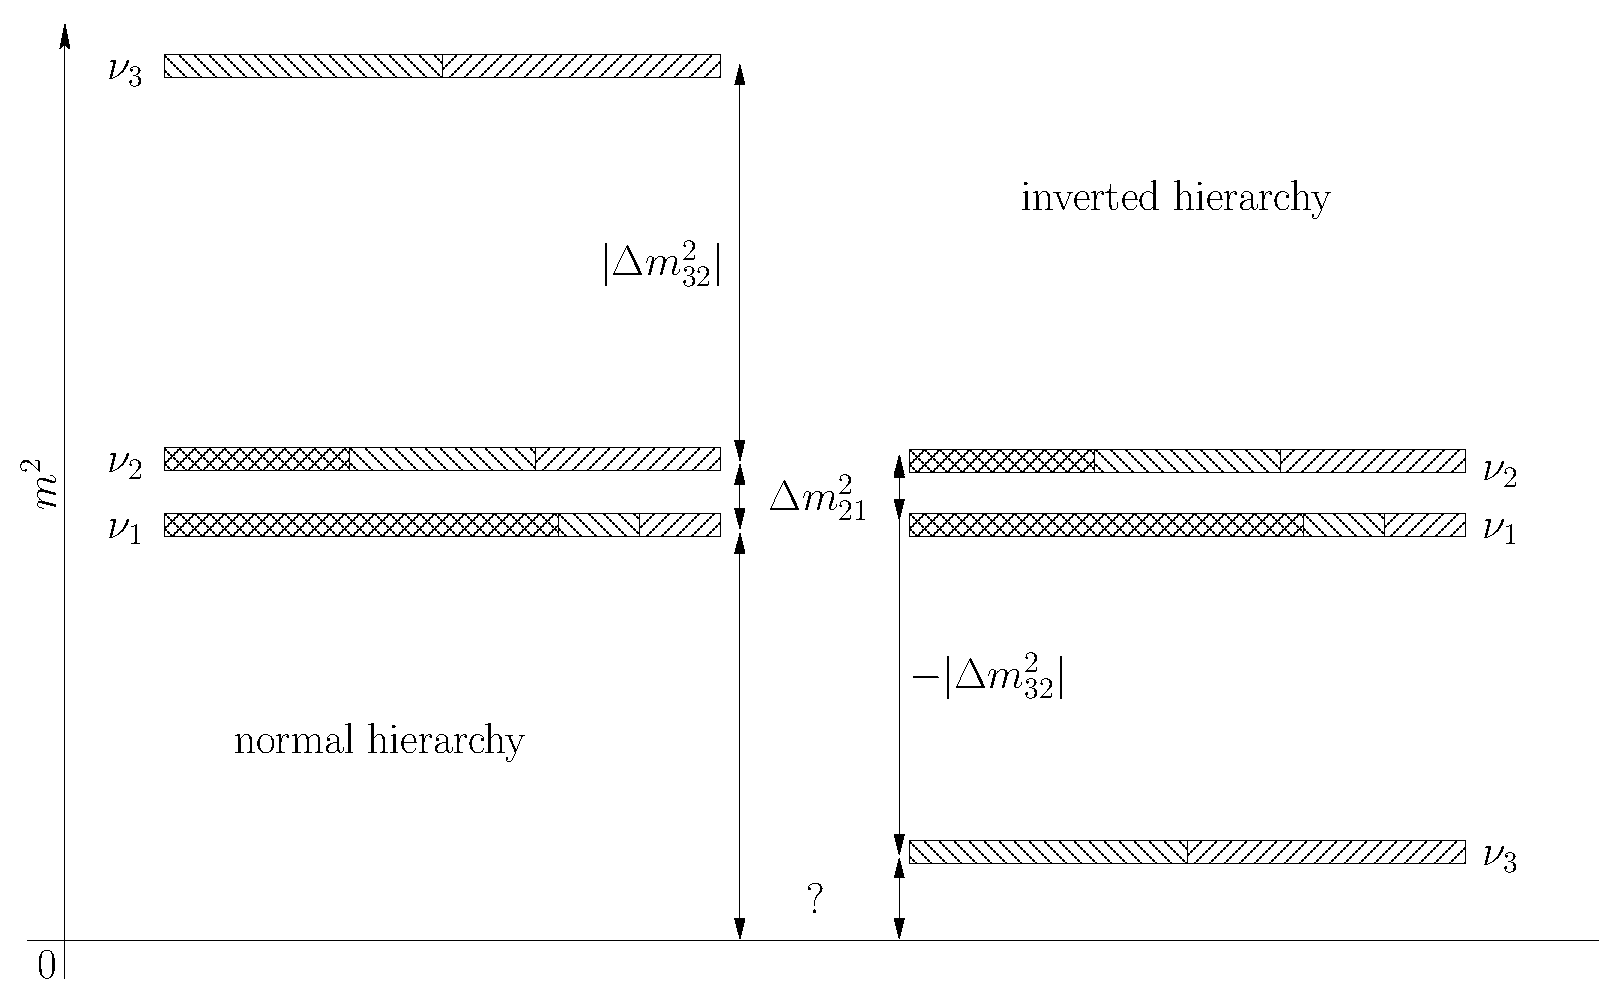
\includegraphics[width=0.8\textwidth]{massHierarchy.eps}  
  \caption{Possible neutrino squared-mass spectra. Oscillation     experiments can neither tell how far above zero the entire spectra     lie, nor the real mass hierarchy.}
  \label{fig:hie}
\end{figure}

\begin{table}[tbhp]
  \centering
  \caption{Summary of the neutrino squared-mass differences and the             mixing parameters based on the 3-neutrino mixing scheme. The suffixes         $_\odot$ and $_{\mbox{atm}}$ stand for the results from solar and         atmosphere experiments, respectively.}
  \label{tab:par}
  \begin{tabular}{lr}\hline\hline
    Parameter & Value \\\hline
    $\sin^{2}2\theta_{12} \approx \sin^{2}2\theta_{\odot}$ &     $0.86^{+0.03}_{-0.04}$ \\
    $\sin^{2}2\theta_{23} \approx \sin^{2}2\theta_{\mbox{atm}}$ &         $>0.92$ (C.L. = 90\%) \\
    $\sin^{2}2\theta_{13}$ & $<0.19$ (C.L. = 90\%) \\
    $\Delta m^{2}_{21}~[10^{-5}\mbox{eV}^{2}]$ & $0.8 \pm 0.3$ \\
    $|\Delta m^{2}_{32}|~[10^{-3}\mbox{eV}^{2}]$ & 1.9 to 3.0         \\\hline\hline
  \end{tabular}
\end{table}

\section{Dirac neutrinos}
\label{sec:dirac}
The observation of neutrino oscillations makes the introduction of neutrino mass terms into the \emph{Standard Model} necessary. In case of free fields of fermions, the Dirac equation can be deduced from the Lagrangian density
\begin{equation}
  \label{eq:deq}
  \mathcal{L} = \bar{\psi} (i\gamma^{\mu}\partial_{\mu}-m) \psi,
\end{equation}
where $\psi$ is the free Dirac field. The first term corresponds to the kinetic energy and the second is the Dirac mass term,
\begin{equation}
  \label{eq:dm}
  \mathcal{L}_D=m_{D}\bar{\psi}\psi.
\end{equation}
Since
\begin{equation}
  \label{eq:2psi}
  \bar{\psi}\psi =  \bar{\psi}     \left(\frac{1+\gamma^5}{2}+\frac{1-\gamma^5}{2}\right)
  \left(\frac{1+\gamma^5}{2}+\frac{1-\gamma^5}{2}\right) \psi =
  \bar{\psi}_{L}\psi_{R}+\bar{\psi}_{R}\psi_{L},
\end{equation}
a right-handed partner of the left-handed neutrino must be introduced in order to prevent the above term vanishing. This particle does not participate the weak interaction hence is called as the sterile neutrino.

To motivate the above mass term, the most straightforward approach is to follow the same procedure as for the electron, \textit{i.e.} the lepton obtains mass by coupling to the Higgs field. The mass term of the electron can be expressed as
\begin{equation}
  \label{eq:dme}
  m_{e}\bar{\psi_e}\psi_{e} = g_{e}\langle       h^{0}\rangle\bar{\psi_e}\psi_{e},
\end{equation}
where $g_e$ is the coupling strength of electron field with Higgs field, $\langle h^{0}\rangle$ is the vacuum expectation value for the Higgs field. Similarly,
\begin{equation}
  \label{eq:dmnu}
  m_{\nu}\bar{\psi_\nu}\psi_{\nu} = g_{\nu}\langle   h^{0}\rangle\bar{\psi_\nu}\psi_{\nu},
\end{equation}
where $g_\nu$ is the coupling strength of neutrino field with Higgs field. Since neutrinos are much lighter than their leptonic partners, the coupling strength of neutrino field with Higgs field should be much smaller than that of electron:
\begin{equation}
  \label{eq:gg}
  g_{\nu} \ll g_{e}.
\end{equation}
By only introducing the Dirac mass term one has to answer the question why neutrinos couple to the Higgs field so weakly compared with their leptonic partners.

\section{Majorana neutrinos}
\label{sec:major}
Theoretically speaking, $\bar{\psi}^{c}\psi^{c}, \bar{\psi}\psi^{c}$ and $\bar{\psi}^{c}\psi$ are also possible mass terms, where $\psi^{c}$ are the charge conjugate of $\psi$. $\bar{\psi}^{c}\psi^{c}$ is equivalent to $\bar{\psi}\psi$. $\bar{\psi}\psi^{c}$ and $\bar{\psi}^{c}\psi$ cannot be the mass terms for electrons or quarks because it destroys or creates two particles of the same charge. But nothing forbids to use them as mass terms for neutrinos because neutrinos have no charge. These mass terms destroy or creates two particles of the same lepton number hence violate lepton number conservation, which is not necessarily to be true as being discussed in section~\ref{sec:sm}.

After abandoning the lepton number conservation a generetic expression of the mass term of one generation of neutrino is
\begin{equation}
  \label{eq:dmm}
  \mathcal{L}_{D+M} = m_{D}(\bar{\psi}_{L}\psi_{R} +   \bar{\psi}^{c}_{L}\psi^{c}_{R}) +
  m_{L}\bar{\psi}_{L}\psi^{c}_{R} +   m_{R}\bar{\psi}^{c}_{L}\psi_{R} + h.c.,
\end{equation}
which can be reframed as
\begin{equation}
  \label{eq:mm}
  \mathcal{L}_{D+M} = (\bar{\psi}_{L},\bar{\psi}^{c}_{L})
  \left(\begin{array}{cc}m_L & m_D \\ m_D & m_R\end{array}\right)
  \left(\begin{array}{c}\psi^{c}_R \\ \psi_R\end{array}\right) + h.c.
\end{equation}
By choosing a orthogonal matrix $\mathcal{U}$ ($\mathcal{U}^{T} \mathcal{U} = 1$) so that
\begin{equation}
  \label{eq:mmat}
  \mathcal{U}^{T}\left(\begin{array}{cc}m_L & m_D \\ m_D &        m_R\end{array}\right)\mathcal{U} = 
  \left(\begin{array}{cc}\epsilon_{1}m_1 & 0 \\ 0 &             \epsilon_{2}m_2\end{array}\right),
\end{equation}
where $m_{1}, m_{2} > 0$, $\epsilon_{1,2}$ indicate the signs of $m_{1}, m_{2}$ and hence equal to $\pm 1$, and defining
\begin{equation}
  \label{eq:mvet}
  (\psi_{1L}, \psi_{2L}) = 
  (\bar{\psi}_{L}, \bar{\psi}^{c}_{L})~ \mathcal{U},
  \left(\begin{array}{c} \psi^{c}_{1R} \\             \psi^{c}_{2R}\end{array}\right) = \mathcal{U}^{T}
  \left(\begin{array}{c} \psi^{c}_{R} \\ \psi_{R} \end{array}\right),
\end{equation}
eq.~\ref{eq:mm} can be rewritten as
\begin{equation}
  \label{eq:m12}
  \mathcal{L}_{D+M} = m_{1}\bar{\psi}_{1L}\psi^{c}_{1R} +   m_{1}\bar{\psi}^{c}_{1R}\psi_{1L} +
  m_{2}\bar{\psi}_{2L}\psi^{c}_{2R} +   m_{2}\bar{\psi}^{c}_{2R}\psi_{2L}.
\end{equation}
Define
\begin{equation}
  \label{eq:mafi}
  \phi_{1} = \psi_{1L} + \epsilon_{1}\psi^{c}_{1R}, 
  \mbox{\ \ \ and \ \ \ }
  \phi_{2} = \psi_{2L} + \epsilon_{2}\psi^{c}_{2R}.
\end{equation}
Eq.~\ref{eq:mm} can be rewritten as
\begin{equation}
  \label{eq:mv}
  \mathcal{L}_{D+M} = m_{1}\bar{\phi}_{1}\phi_{1} + m_{2}\bar{\phi}_{2}\phi_{2}
\end{equation}
It is easy to find out that
\begin{equation}
  \label{eq:mach}
  \phi^{c}_{k} = (\psi_{kL})^{c} + \epsilon_{k}(\psi^{c}_{kR})^{c} = \epsilon_{k}\phi_{k}, ~~~ (k=1,2)
\end{equation}
\textit{i.e.} $\psi$ is its own anti-particle, and hence of Majorana type.

In case that $m_{R}$ is very heavy, $m_{L} = 0$ and $m_{D} \approx \mathcal{O}(m_{e})$, we have
\begin{equation}
  \label{eq:seesaw}
  m_{1} = \frac{m^{2}_{D}}{m_{R}}\ll m_{D},  \mbox{\ \ \ and \ \ \ }   m_{2} = m_{R}(1+\frac{m^{2}_{D}}{m^{2}_{R}}) \approx m_{R} \gg m_{D}.
\end{equation}
\textit{i.e.} if there exists a very heavy Majorana neutrino $\phi_2$, the other Majorana neutrino would be much lighter than $m_e$. This is so-called seesaw machenism.

To sum up, Majorana mass terms should be taken into account in general as well as Dirac mass terms. For fermions carrying charge or similar quantum numbers the former mass terms are forbidden, while this is not the case for neutrinos. Majorana neutrinos $\phi_{1}, \phi_{2}$ can be constructed out of Dirac fields. By using seesaw mechanism the tiny neutrino mass can be explained naturally.

\section{Neutrinoless double beta decay}
\label{sec:0n2b}
If neutrinos are of Majorana type the two neutrinos from double beta decay ($2\nu\beta\beta$) as shown in eq.~\ref{eq:2nu2b} may annihilate with each other. This is the so-called neutrinoless double beta decay ($0\nu\beta\beta$) as shown in eq.~\ref{eq:0nu2b}:
\begin{eqnarray}
  2\nu\beta\beta: &(Z,A)& \rightarrow (Z+2,A) + 2e^{-} + 2\bar{\nu}_{e}, \\\label{eq:2nu2b}
  0\nu\beta\beta: &(Z,A)& \rightarrow (Z+2,A) + 2e^{-}, \label{eq:0nu2b}
\end{eqnarray}
where $Z$ is the charge of the nucleus and $A$ is the atomic number. The Feynman Diagram of both processes are shown in Fig.~\ref{fig:2bdecay}.
\begin{figure}[tbhp]
  \centering
  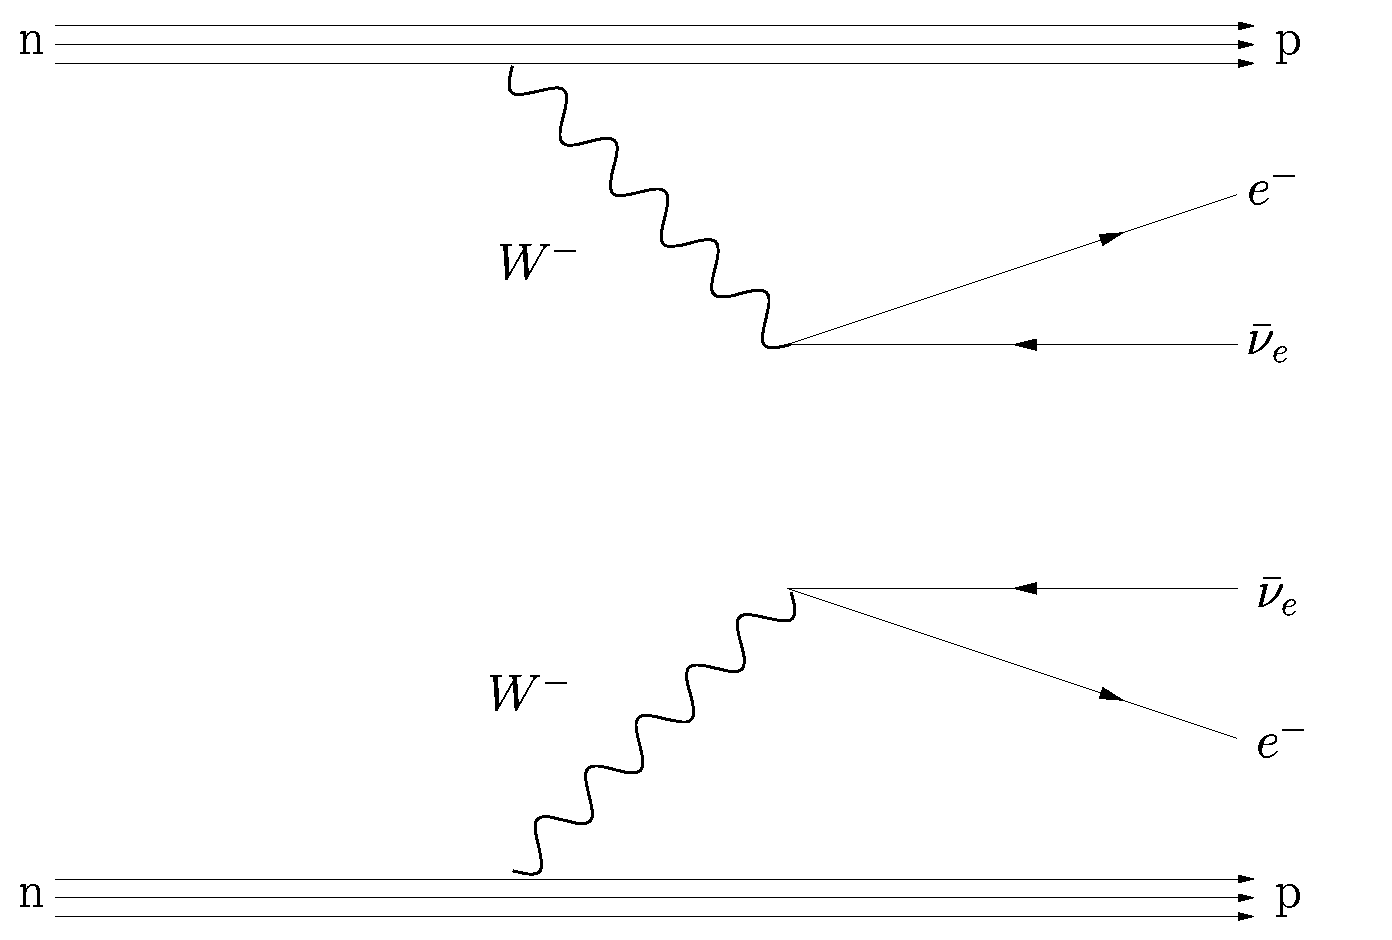
\includegraphics[width=0.45\textwidth]{FD2nu2b.eps} \hfil
  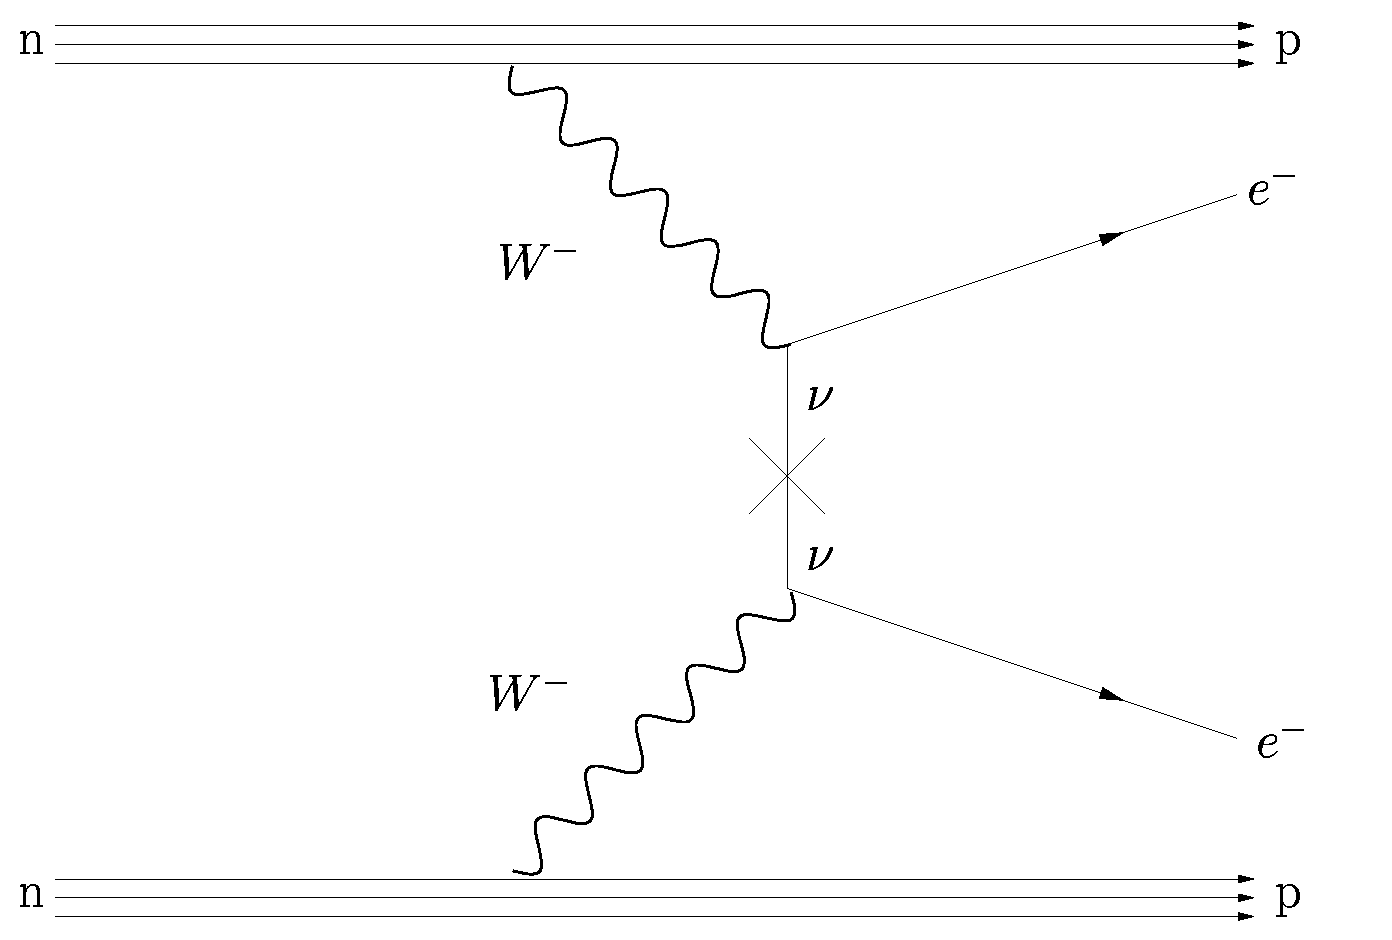
\includegraphics[width=0.45\textwidth]{FD0nu2b.eps}  
  \caption{Feynman diagrams of double beta decay with and without the         emittance of the neutrino.}
  \label{fig:2bdecay}
\end{figure}

\subsection{Double beta decay with neutrinos}
\label{sec:2n2b}
The study of double beta decay started in 1935~\cite{Goe35} when Maria Goeppert-Mayer applied Fermi's beta decay theory to calculate the process as shown in eq.~\ref{eq:2nu2b} as a second order effect. Her motivation had nothing to do with neutrinos, but rather was concerned with the stability of various even-even nuclei over geological time. These nuclei, consisting of even numbers of protons and neutrons, were forbidden from decaying into their nearest neighbor odd-odd nuclei by energy conservation, but could decay into their next nearest neighbors, as shown in Fig.~\ref{fig:ee2oo}. It is known now that more than 60 naturally occurring isotopes are capable of undergoing double-beta decay. Only ten of them were observed to decay. They are $^{48}$Ca, $^{76}$Ge, $^{82}$Se, $^{96}$Zr, $^{100}$Mo, $^{116}$Cd, $^{128}$Te, $^{130}$Te, $^{150}$Nd, and $^{238}$U. A comprehensive list of the decay modes and the corresponding lifetime for each isotope can be found in the latest \emph{Review of Particle Physics}~\cite{PDG07}.
\begin{figure}[tbhp]
  \centering
  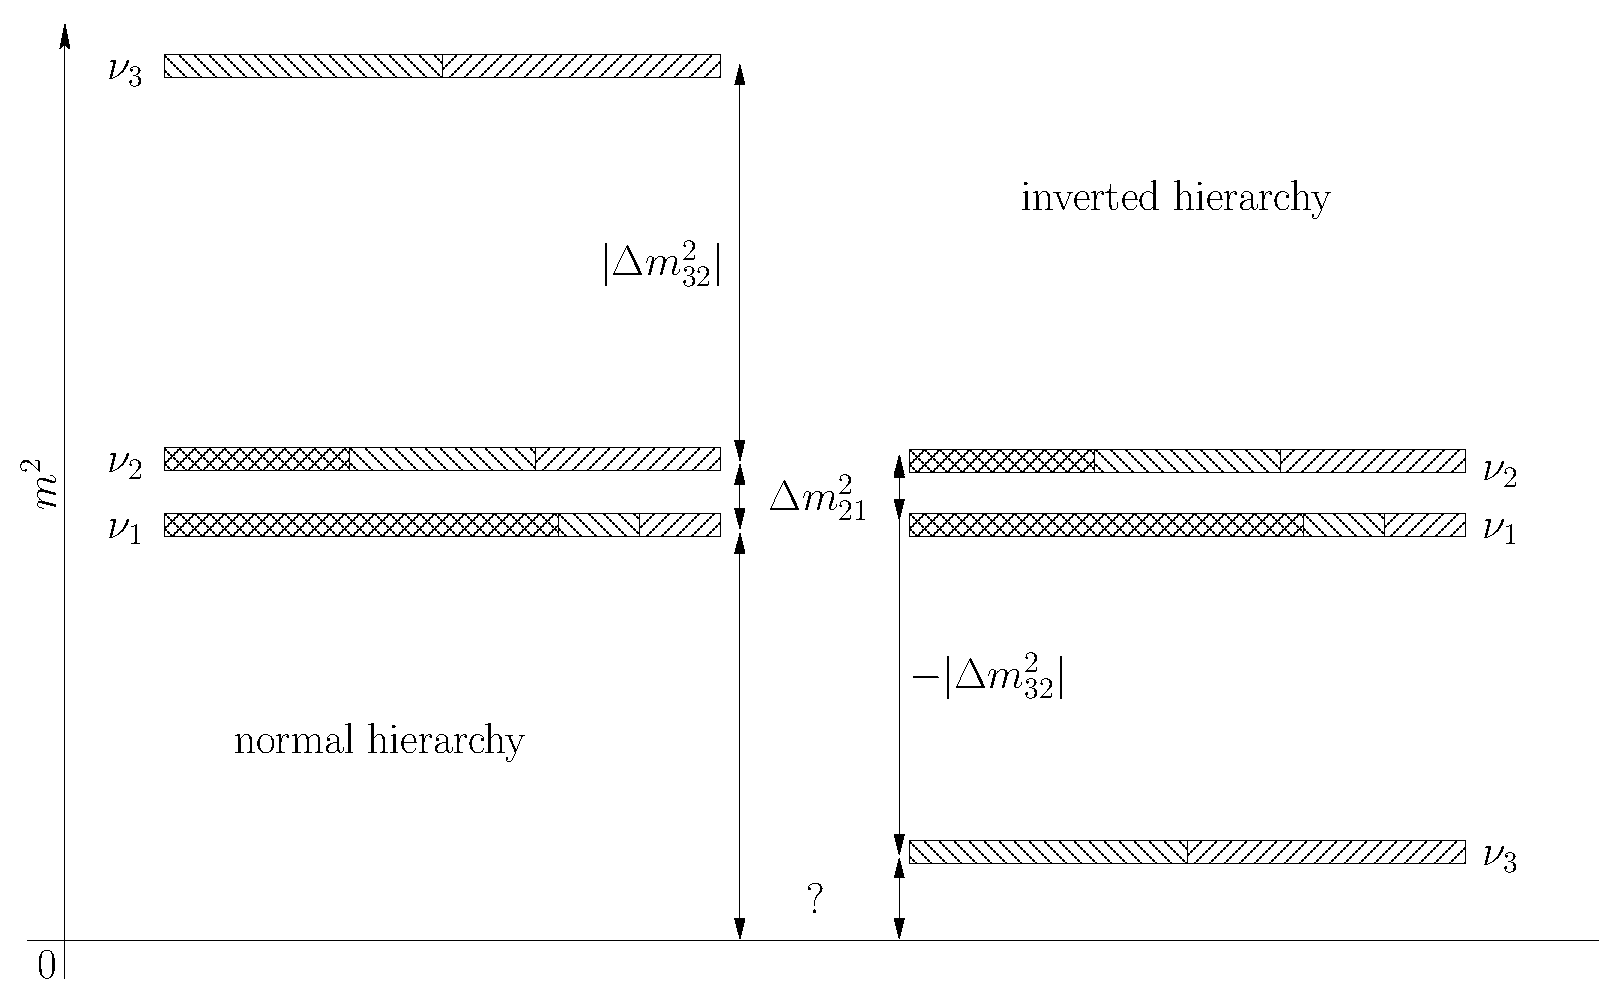
\includegraphics[width=0.8\textwidth]{massHierarchy.eps}  
  \caption{Energy scheme for the double beta decay from parent nucleus
$^{A}X$ to daughter nucleus $^{A}Y$. The single beta decay to the
intermediate isotope $^{A}T$ is forbidden by the energy conservation.}
  \label{fig:ee2oo}
\end{figure}

\subsection{Rate of neutrinoless double beta decay}
\label{sec:0n2brate}
The study of neutrinoless double beta decay started several years later~\cite{Rac37,Fur37} when W. H. Furry showed that Majorana's symmetrical theory of neutrino and anti-neutrino could give rise to a neutrinoless mode of double beta decay. Prior to the discovery of parity non-conservation, the lifetime of neutrinoless double beta decay was calculated incorrectly. The understanding of double beta decay changed profoundly when parity non-conservation was discovered in 1957 and the two-component theory of the neutrino was developed. According to the two-component theory the probability for neutrinoless double beta decay via Furry's mechanism is zero because the neutrino emitted in the first beta decay is in the wrong helicity state to stimulate a second beta decay process. The observation of neutrino oscillations changed the picture once again. The rate of neutrinoless double beta decay can be expressed as
\begin{equation}
  \label{eq:0nura}
  1/T^{0\nu}_{1/2} = \sum_{\text{spins}} \int |Z_{0\nu}|^{2} \delta(E_{e1} + E_{e2} + Q_{\beta\beta}) \frac{d^{3}p_{e1}}{(2\pi)^{3}} \frac{d^{3}p_{e2}}{(2\pi)^{3}},
\end{equation}
where $Q_{\beta\beta}$ is the Q-value of the decay, $E_{e1}, E_{e2}, p_{e1}, p_{e2}$ are the energies and momenta of the outgoing electrons and $Z_{0\nu}$ is the transition amplitude. $Z_{0\nu}$ contains both leptonic and hadronic parts. Taking into account the neutrino mixing the leptonic part is of the form
\begin{equation}
  \label{eq:leppar}
  \contraction{\sum_{k}\bar{e}(x)\gamma_{\mu}(1-\gamma_{5})U_{ek}}
  {\phi}{{}_{k}(x)\bar{e}(y)\gamma_{\nu}(1-\gamma_{5})U_{ek}}{\phi}
  \sum_{k}\bar{e}(x)\gamma_{\mu}(1-\gamma_{5})U_{ek}\phi_{k}(x)
  \bar{e}(y)\gamma_{\nu}(1-\gamma_{5})U_{ek}\phi_{k}(y).
\end{equation}
Assuming only the exchange of three light neutrinos, the leptonic part is proportional to 
\begin{equation}
  \label{eq:effmass}
  \langle m_{\nu_{e}} \rangle \equiv \left| \sum_{k}m_{k}U^{2}_{ek} \right| = \left| m_{1}|U_{e1}|^{2} + m_{2}|U_{e2}|^{2}e^{i(\alpha_{2}-\alpha_{1})} + m_{3}|U_{e3}|^{2}e^{-i(\alpha_{1}+2\delta)} \right|,
\end{equation}
where $\langle m_{\nu_{e}} \rangle$ is called the effective Majorana neutrino mass. The rate of neutrinoless double beta decay can be expressed in term of the effective Majorana neutrino mass as
\begin{equation}
  \label{eq:0nurate}
  1/T^{0\nu}_{1/2} = G_{0\nu}(Q,Z) |\mathcal{M}_{0\nu}|^{2} \langle m_{\nu_{e}} \rangle^{2},
\end{equation}
where $G_{0\nu}(Q,Z)$ is the phase space factor, $\mathcal{M}_{0\nu}$ denotes the nuclear matrix elements which describe the hadronic part of the decay. 

If the neutrino squared-mass spectrum is of the normal order, as shown in the left plot of Fig.~\ref{fig:hie}, the effective Majorana neutrino mass could be invisibly small. Because the terms in eq.~\ref{eq:effmass} can cancel each other out if the CP-violation phases $\alpha_{1}, \alpha_{2}$ and $\delta$ take some special values. Fig.~\ref{fig:effmvmm} taken from Ref.~\cite{Mer06} shows the effective Majorana neutrino mass as a function of the lightest neutrino mass. The mixing angle $\theta_{13}$ is assumed to be zero. The light band corresponds to the inverted mass hierarchy, the dark band to the normal mass hierarchy. An experiment sensitive to $\langle m_{\nu_{e}} \rangle \sim 10$meV has an excellent chance to seeing a signal in case of inverted mass hierarchy. And if the observed $\langle m_{\nu_{e}} \rangle$ is far below $10$meV the inverted mass hierarchy can be ruled out.
\begin{figure}[tbhp]
  \centering
  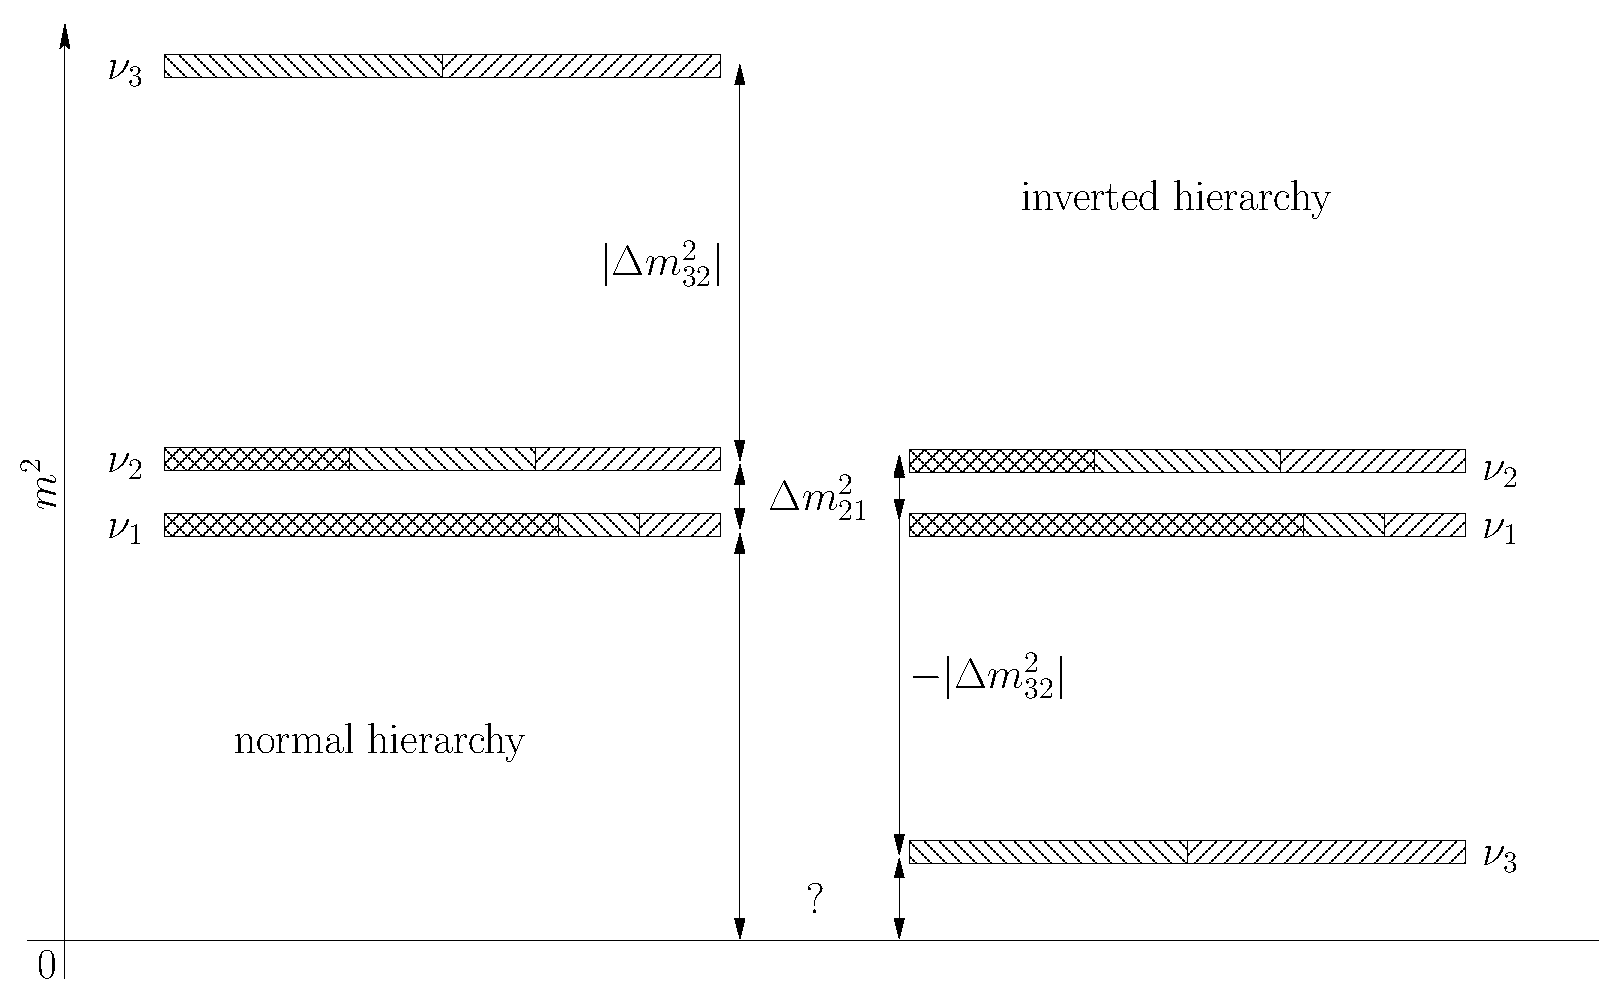
\includegraphics[width=0.8\textwidth]{massHierarchy.eps}  
  \caption{The effective Majorana neutrino mass as a function of the lightest neutrino mass, m. The mixing angle $\theta_{13}$ is assumed to be zero. The light band corresponds to the inverted mass hierarchy, the dark band to the normal mass hierarchy. the inner/outer bands correspond to calculations without/with the $3\sigma$-uncertainties on the oscillation parameters. }
  \label{fig:effmvmm}
\end{figure}

\subsection{Double beta decay experiments}
\label{sec:genremark}
Q-value, nuclear matrix, natural abundance, background, efficiency ...

comparison between different double beta decay experiments.

\subsection{Neutrinoless double beta decay of $^{76}$Ge}
\label{sec:ge76}

advantage of $^{76}$Ge.

IGEX and Heidelberg-Moscow.

\section{Other aspects of neutrino physics}
\label{sec:others}

\subsection{Seesaw mechanism}
\label{sec:seesaw}
the problems of seesaw mechanism

\subsection{Neutrino pair production}
\label{sec:pair}
the cross sections are different if neutrinos are of different type.

\subsection{Neutrino magnetic moment}
\label{sec:mag}
if neutrino has magnetic moment, it cannot be of Majorana type.

\subsection{Neutrinos in astrophysics}
\label{sec:astro}
mass and number of types of neutrinos



%%% Local Variables:
%%% mode:latex
%%% TeX-master: "thesis"
%%% End:
